
%%%%%%%%%%%%%%%%%%%%%%%%%%%%%%%%%%%%%%%%%%%%%%%%%%%%%%%%%%%%
%%%%%%%%%%%%%%%%%%%%%%% preamble %%%%%%%%%%%%%%%%%%%%%%%%%%%
%%%%%%%%%%%%%%%%%%%%%%%%%%%%%%%%%%%%%%%%%%%%%%%%%%%%%%%%%%%%

\documentclass[10pt,letterpaper]{article}

\usepackage{opex3}
\usepackage{times}
\usepackage{graphicx}
\graphicspath{{./images/}}
\usepackage{epstopdf}
\usepackage{amsmath}
\usepackage{amssymb}
\usepackage{url}
\usepackage{bm}
\usepackage{enumerate}
\usepackage[]{todonotes} % Add option [disable] to hide all todo notes.
\usepackage{xfrac}
\usepackage{paralist}
\usepackage{cite}

%\usepackage{ae} %%for Computer Modern fonts

\usepackage{hyperref}
\hypersetup{pdfborder={0 0 0}}

%
% subfiles is useful for having the abstract (and possible other
% sections/chapters) as separate files.
%
\usepackage{subfiles}

\usepackage[]{siunitx}

%
% The cleveref package seems very cool but currently it doesn't support hebrew
% (babel) very well, so I just use if for single references.
% As a work around I redefine the number definition as suggested in:
% http://tex.stackexchange.com/questions/118235/using-the-cleveref-package-with-hebrew-and-babel
%
\usepackage[capitalise]{cleveref}
\makeatletter
\def\@@number#1{#1}
\makeatother

\DeclareMathAlphabet\mathbfcal{OMS}{cmsy}{b}{n}


%
% Some new commands I use in this text
%
% Note:
% Nice curly font is {\bm{\mathcal{D}}}
%
\newcommand{\Grad}[1]{\bm{\triangledown_{#1}}}
\newcommand{\abbrev}[1]{\rm{#1}}
\newcommand{\argmin}{\mathrm{arg}\min}
\newcommand{\curly}[1]{\left\{#1\right\}}
\newcommand{\roundy}[1]{\left(#1\right)}
\newcommand{\recty}[1]{\left[#1\right]}
\newcommand{\PartDeriv}[2]{\frac{\partial{#1}}{\partial{#2}}}
\newcommand{\vect}[1]{\bm{#1}}
\newcommand{\mat}[1]{\bm{#1}}
\newcommand{\transpose}[1]{{#1}^\intercal}
\newcommand{\derivsym}[1]{\,d{#1}}
\newcommand{\yoavcomment}[1]{}
\renewcommand{\yoavcomment}[1]{#1} % Comment to remove images

%
% Used symbols (only partial for now...)
%
\newcommand{\OpSphere}{\mathbfcal{S}}
\newcommand{\OpRot}{\mathbfcal{R}}
\newcommand{\OpDistance}{\bm{D}}
\newcommand{\OpCumsum}{\mathbfcal{C}}
\newcommand{\OpInt}{\mathbfcal{I}}
\newcommand{\OpCamera}{\mathbfcal{P}}
\newcommand{\MaskSun}{\mathbfcal{M}}
\newcommand{\Laplacian}{\mathbfcal{L}}
\newcommand{\OpDiag}[1]{\mathbb{D}\left\{#1\right\}}
\newcommand{\DistSet}{\mathcal{C}}
\newcommand{\DistUnknown}{\vect{n}}
\newcommand{\DistEstimated}{\hat{\vect{n}}}
\newcommand{\CostFunc}[1]{E(#1)}

%
% For the title
%
\newcommand\authnote[1]{\textsuperscript{\normalfont#1}}
\newcommand\affilnote[1]{\textsuperscript{\normalfont#1}}
\providecommand\textsuperscript[1]{$^{#1}$}

%%%%%%%%%%%%%%%%%%%%%%%%%%%%%%%%%%%%%%%%%%%%%%%%%%%%%%%%%%%%
%%%%%%%%%%%%%%%%%%%%%%% begin %%%%%%%%%%%%%%%%%%%%%%%%%%%%%%
%%%%%%%%%%%%%%%%%%%%%%%%%%%%%%%%%%%%%%%%%%%%%%%%%%%%%%%%%%%%

\begin{document}

%%%%%%%%%%%%%%%%%%%%%%%%%%%%%%%%%%%%%%%%%%%%%%%%%%%%%%%%%%%%
%%%%%%%%%%%%%%%%%% title page information %%%%%%%%%%%%%%%%%%
%%%%%%%%%%%%%%%%%%%%%%%%%%%%%%%%%%%%%%%%%%%%%%%%%%%%%%%%%%%%

\title{Multi sky-view\\ 3D aerosol distribution recovery}

\author{Amit~Aides,\authnote{1*} Yoav~Y.~Schechner,\authnote{1}
  Vadim~Holodovsky\authnote{1} and Michael~J.~Garay\authnote{2}}

\address{\affilnote{1}Electrical Engineering Department, Technion - Israel Institute of Technology, Haifa 32000, Israel\\
  \affilnote{2}Jet Propulsion Laboratory, California Institute of
  Technology, Pasadena, CA 91109, USA}

\email{\authnote{*}amitibo@tx.technion.ac.il} %% email address is required

% \homepage{http:...} %% author's URL, if desired

%%%%%%%%%%%%%%%%%%%%%%%%%%%%%%%%%%%%%%%%%%%%%%%%%%%%%%%%%%%%
%%%%%%%%%%%%%%%%%%% abstract and OCIS codes %%%%%%%%%%%%%%%%
%%%%%%%%%%%%%%%%%%%%%%%%%%%%%%%%%%%%%%%%%%%%%%%%%%%%%%%%%%%%

%% [use \begin{abstract*}...\end{abstract*} if exempt from copyright]

\begin{abstract}
  Aerosols effect climate, health and aviation.  Currently, their
  retrieval assumes a plane-parallel atmosphere and solely vertical
  radiative transfer (RT). We propose a principle to estimate the
  aerosol distribution as it really is: a three dimensional (3D)
  volume, using visible light.  The principle is a type of
  tomography. The process involves wide angle integral imaging of the
  sky on a very large scale.  We formulate an image formation model
  based on 3D RT. Model inversion is done using optimization methods,
  exploiting a closed-form gradient which we derive for the model-fit
  cost function.  The tomography model is distinct, as the radiation
  source is unidirectional and uncontrolled, while off-axis scattering
  dominates the images.
\end{abstract}

\ocis{(000.0000)
  General.} % REPLACE WITH CORRECT OCIS CODES FOR YOUR ARTICLE

%%%%%%%%%%%%%%%%%%%%%%%%%%%%%%%%%%%%%%%%%%%%%%%%%%%%%%%%%%%%
%%%%%%%%%%%%%%%%%%%%%%% References %%%%%%%%%%%%%%%%%%%%%%%%%
%%%%%%%%%%%%%%%%%%%%%%%%%%%%%%%%%%%%%%%%%%%%%%%%%%%%%%%%%%%%

%\bibliography{article}{} \bibliographystyle{osajnl}

\begin{thebibliography}{10}
\newcommand{\enquote}[1]{``#1''}

\bibitem{Stern2006}
A.~Stern and B.~Javidi, \enquote{{Three-dimensional image sensing,
  visualization, and processing using integral imaging},} Proceedings of the
  IEEE \textbf{94} (2006).

\bibitem{kim}
J.~Kim, D.~Lanman, Y.~Mukaigawa, and R.~Raskar, \enquote{{Descattering
  transmission via angular filtering},} in \enquote{Proc. ECCV' 10,}
  (Springer-Verlag, Berlin, Heidelberg, 2010), pp. 86--99.

\bibitem{Ng1948}
M.~Levoy, R.~Ng, A.~Adams, M.~Footer, and M.~Horowitz, \enquote{{Light field
  microscopy},} ACM Transactions on Graphics (TOG) \textbf{25}, 924----934
  (2006).

\bibitem{Dayan2008}
U.~Dayan, B.~Ziv, T.~Shoob, and Y.~Enzel, \enquote{{Suspended dust over
  southeastern Mediterranean and its relation to atmospheric circulations},}
  International Journal of Climatology \textbf{924}, 915--924 (2008).

\bibitem{kalashnikova}
O.~V. Kalashnikova, M.~J. Garay, A.~B. Davis, D.~J. Diner, and J.~V.
  Martonchik, \enquote{{Sensitivity of multi-angle photo-polarimetry to
  vertical layering and mixing of absorbing aerosols: Quantifying measurement
  uncertainties},} Journal of Quantitative Spectroscopy and Radiative Transfer
  \textbf{112}, 2149--2163 (2011).

\bibitem{Mishchenko2007}
M.~I. Mishchenko and I.~V. Geogdzhayev, \enquote{{Satellite remote sensing
  reveals regional tropospheric aerosol trends.}} Optics express \textbf{15},
  7423--38 (2007).

\bibitem{Martonchikc}
J.~Martonchik, D.~D.~J. Diner, J.~M. David, R.~Kahn, T.~P. Ackerman, M.~M.
  Verstraete, B.~Pinty, and H.~R. Gordon, \enquote{{Techniques for the
  Retrieval of Aerosol Properties over Land and Ocean Using Multi-angle
  Imaging},} IEEE Trans. on Geoscience and Remote Sensing \textbf{36},
  1212--1227 (1998).

\bibitem{Namer2009}
E.~Namer, S.~Shwartz, and Y.~Y. Schechner, \enquote{{Skyless polarimetric
  calibration and visibility enhancement.}} Optics express \textbf{17}, 472--93
  (2009).

\bibitem{Bluestone2001}
a.~Bluestone, G.~Abdoulaev, C.~Schmitz, R.~Barbour, and A.~Hielscher,
  \enquote{{Three-dimensional optical tomography of hemodynamics in the human
  head},} Optics express \textbf{9}, 272--86 (2001).

\bibitem{messer}
H.~Messer, A.~Zinevich, and P.~Alpert, \enquote{{Environmental sensor networks
  using existing wireless communication systems for rainfall and wind velocity
  measurements},} IEEE Instrumentation \& Measurement Magazine \textbf{15},
  32--38 (2012).

\bibitem{gregson}
J.~Gregson, M.~Krimerman, M.~B. Hullin, and W.~Heidrich, \enquote{{Stochastic
  tomography and its applications in 3D imaging of mixing fluids},} ACM Trans.
  Graph. \textbf{31}, 52:1----52:10 (2012).

\bibitem{Cosofret2009}
B.~R. Cosofret, D.~Konno, A.~Faghfouri, H.~S. Kindle, C.~M. Gittins, M.~L.
  Finson, T.~E. Janov, M.~J. Levreault, R.~K. Miyashiro, and W.~J. Marinelli,
  \enquote{{Imaging sensor constellation for tomographic chemical cloud
  mapping},} Applied optics \textbf{48}, 1837--52 (2009).

\bibitem{Aviles2011}
J.~A. Aviles, \enquote{{The Development and Validation of a First Generation
  X-Ray Scatter Computed Tomography Algorithm for the Reconstruction of
  Electron Density Breast Images Using Monte Carlo Simulation},} Ph.D. thesis
  (2011).

\bibitem{Cornette1995}
W.~M. Cornette and J.~G. Shanks, \enquote{{Physically reasonable analytic
  expression for the single-scattering phase function: errata.}} Applied optics
  \textbf{34}, 641 (1995).

\bibitem{Levi1980}
L.~Levi, \emph{{Applied Optics}} (John Wiley \& Sons, Inc., 1980).

\bibitem{devroye1986sample}
L.~Devroye, \enquote{{Sample-based non-uniform random variate generation},} in
  \enquote{Proceedings of the 18th conference on Winter simulation,}  (ACM,
  1986), pp. 260--265.

\bibitem{Hong2004}
S.-H. Hong, J.-S. Jang, and B.~Javidi, \enquote{{Three-dimensional volumetric
  object reconstruction using computational integral imaging.}} Optics express
  \textbf{12}, 483--91 (2004).

\bibitem{marshak20053d}
A.~Marshak and A.~Davis, \emph{{3D Radiative Transfer in Cloudy Atmospheres}},
  Physics of Earth and Space Environments (Springer, 2005).

\bibitem{BBradiance}
M.~Charity, \enquote{{Blackbody color datafile},}  (2001), \url{http://www.vendian.org/mncharity/dir3/blackbody/UnstableURLs/bbr\_color.html}.

\bibitem{sun_composition}
Wikipedia, \enquote{{Sunlight --- Wikipedia\{,\} The Free Encyclopedia},}  (2012), \url{http://en.wikipedia.org/w/index.php?title=Sunlight\&oldid=502554571}.

\bibitem{Martonchik2009}
J.~V. Martonchik, R.~A. Kahn, and D.~J. Diner, \enquote{{Retrieval of aerosol
  properties over land using MISR observations},} in \enquote{Satellite Aerosol
  Remote Sensing over Land,} , A.~A. Kokhanovsky and G.~Leeuw, eds. (Springer
  Berlin Heidelberg, 2009), pp. 267--293.

\bibitem{BFGS}
C.~Zhu, R.~H. Byrd, P.~Lu, and J.~Nocedal, \enquote{{Algorithm 778: L-BFGS-B:
  Fortran subroutines for large-scale bound-constrained optimization},} ACM
  Trans. Math. Softw. \textbf{23}, 550--560 (1997).

\end{thebibliography}

%%%%%%%%%%%%%%%%%%%%%%%%%%%%%%%%%%%%%%%%%%%%%%%%%%%%%%%%%%%%
%%%%%%%%%%%%%%%%%%%%%%%%%%% body %%%%%%%%%%%%%%%%%%%%%%%%%%%
%%%%%%%%%%%%%%%%%%%%%%%%%%%%%%%%%%%%%%%%%%%%%%%%%%%%%%%%%%%%

\section{Introduction}
\label{sec:intro}

Optical lightfield and integral imaging~\cite{Stern2006,kim,Ng1948}
sample the optical radiance distribution in location and
direction. These are mainly used in small-scale setups. This paper
deals with a far larger scale, to estimate scatterer 3D spatial
distribution in the sky.  The atmosphere allows light to pass through
in multiple locations and directions. Light is affected by this
medium. Therefore, in this paper we lay out a principle to recover
this 3D distribution using measured and modeled light-fields
(Fig.~\ref{fig:groundgrid}).
\begin{figure*}[t!]
  \begin{center}
    \yoavcomment{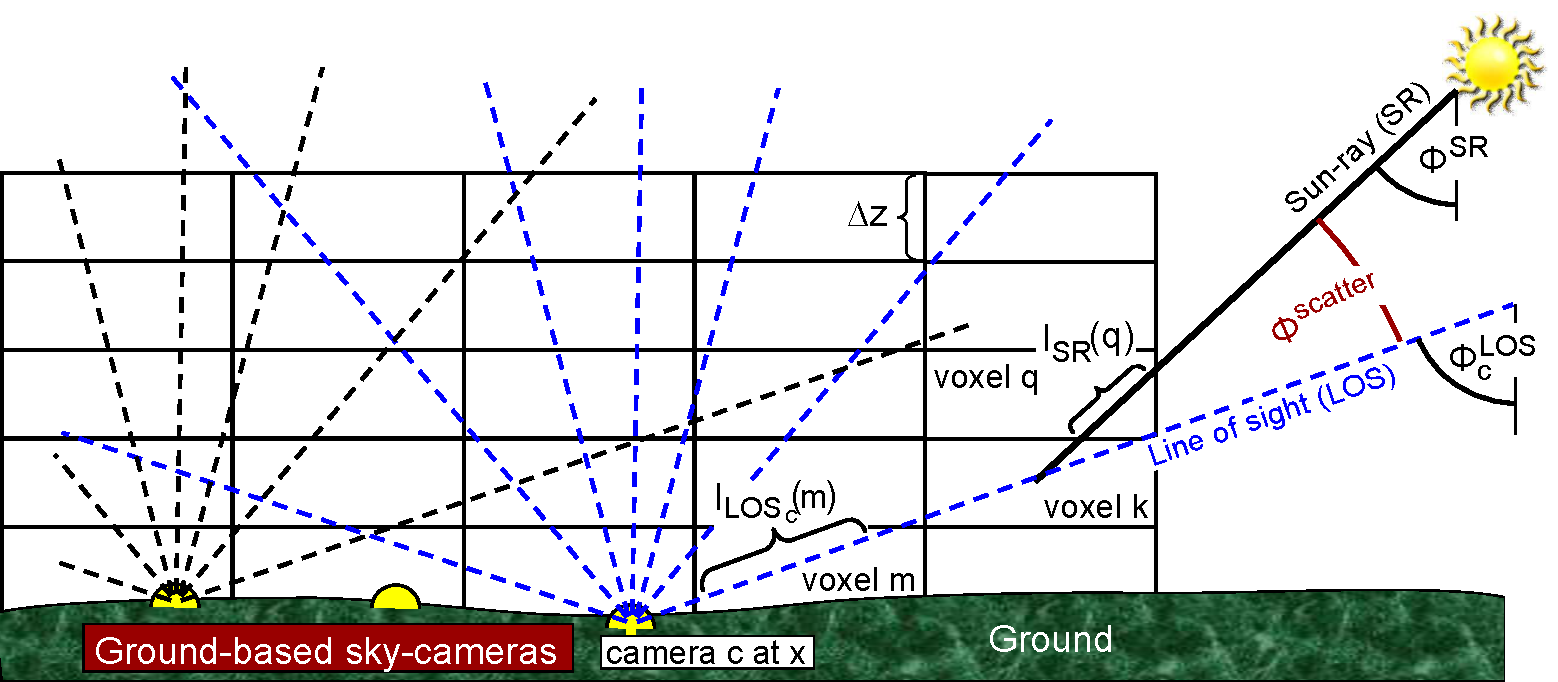
\includegraphics[width=\linewidth]{images/groundtomog24.pdf}}
  \end{center}
  \caption{\small Lightfield imaging through a volumetric distribution
    in the atmosphere, using ground-based cameras.}
  \label{fig:groundgrid}
\end{figure*}
3D recovery of this medium has direct implications to various
scientific communities that either rely on remotely-sensed imagery,
study the atmosphere, or overcome the medium to see beyond. These
include meteorology, atmospheric sciences, volcanology, and
climatology.  Aerosol retrieval is important for understanding climate
evolution~\cite{Dayan2008,kalashnikova} and monitoring air
quality. Mapping aerosol density is significant to aviation safety,
which needs real time assessment of conditions and visibility around
flight paths.

In remote sensing~\cite{Mishchenko2007}, imaging through air is
associated with {\em atmospheric correction}, based on {\em aerosol
  retrieval}. In this discipline, the atmosphere is often assumed to
be plane-parallel, using one-dimensional vertical RT. Consequently
state-of-the-art aerosol retrieval is done in distinct large lateral
blocks~\cite{Martonchikc} with limited height
resolution~\cite{kalashnikova}. We, however, seek 3D
recovery. Atmospheric correction is related to
dehazing~\cite{Namer2009}. In this paper, however, the medium itself,
at all relevant altitudes is the object of interest.


We rely on sky imaging from multiple directions and locations. Such
projection is similar to tomography in other scientific
domains~\cite{Bluestone2001}. However, the situation here is
distinct. Most tomography setups have a controlled and/or
multidirectional radiation source~\cite{Bluestone2001,messer}. In
contrast, our source is the uncontrolled, unidirectional
Sun. Moreover, typical tomography relies on a linear
model~\cite{gregson}: the pixel value is a linear combination of
components along a line of sight (LOS), or a multiplicative
combination (linearized by a logarithm). Linear tomography can detect
gases~\cite{Cosofret2009}, which absorb UV or IR radiation. However,
aerosol attenuation of visible light is typically dominated by {\em
  scattering}, rather than absorption. Since the radiation source is
single and fixed in space and time, we cannot rely on direct
illumination for tomographic recovery of attenuation
fields~\cite{Aviles2011}. We may only use sunlight scattered into the
LOS. The model is {\em nonlinear, yet tractable}. We model passive
optical tomographic imaging of 3D atmospheric scatterer distributions
in cloudless conditions. Then, we solve this tomography problem, to
recover the distribution. Recovery is formulated as an optimization
that minimizes a cost function. We derive the gradient of this cost
function, to enable efficient optimization.




%%%%%%%%%%%%%%%%%%%%%%%%%%%%%%%%%%%%%%%%%%%%%%%%%%%%%%%%%%%%
%%%%%%%%%%%%%%%%%%%%%%%%%%%%%%%%%%%%%%%%%%%%%%%%%%%%%%%%%%%%

\section{Theoretical Background}
\label{sec:theor-backgr}

\noindent {\bf Extinction}: Sun rays (SR) irradiate a small volume
that includes particles of a certain type.  Each particle has an {\em
  extinction cross section} for interacting with the irradiance. For
an aerosol the cross section is denoted $\sigma^{\rm aerosol}$.  The
aerosol density is $n$. Per unit volume, the {\em extinction
  coefficient} due to aerosols is $\beta^{\rm aerosol}= \sigma^{\rm
  aerosol} n$. In addition, the atmosphere contains air molecules.
The extinction coefficient due to the molecules is $\beta^{\rm air}$.
The volume has infinitesimal length $dl$. Then, the relative portion
of extinct SR irradiance is the unitless differential optical depth,
$d\tau= (\beta^{\rm aerosol}+\beta^{\rm air}) dl$.  The {\em optical
  depth} aggregates in extended propagation:
\begin{align}
  \tau= \int d\tau=\int (\beta^{\rm aerosol}+\beta^{\rm air}) dl =\int
  (\sigma^{\rm aerosol} n +\beta^{\rm air}) dl = \tau^{\rm air}+ \int
  \sigma^{\rm aerosol} n dl \;,
  \label{eq:tau}
\end{align}
where $\tau^{\rm air}=\int \beta^{\rm air} dl$.  Through an
attenuating atmosphere, the {\em transmittance} exponentially decays
with the optical depth:
\begin{align}
  t=\exp(-\tau) \;.
  \label{eq:beer-lambert}
\end{align}

\noindent {\bf Scattering}: Interaction of a single particle with the
irradiance is by absorption and scattering. The weight of scattering
(to all directions), relative to the total extinction is given by the
unitless {\em single scattering albedo} of the particle. For an
aerosol, the single scattering albedo is denoted $\varpi^{\rm
  aerosol}$.  The {\em scattering coefficient} due to aerosols in the
volume is
\begin{align}
  \alpha^{\rm aerosol}= \varpi^{\rm aerosol}\beta^{\rm aerosol}
  =\varpi^{\rm aerosol} \sigma^{\rm aerosol} n \;.
  \label{eq:alph}
\end{align}
The angular distribution of scattering by an aerosol is determined by
a {\em phase function} $P^{\rm aerosol}$, which is normalized: its
integral over all solid angles is unit. Part of the light scatters
towards a camera's LOS, as illustrated in \cref{fig:groundgrid}. The
angle between the SR and LOS is the scattering angle $\Phi^{\rm
  scatter}$. The {\em angular scattering coefficient} due to aerosols
is
\begin{align}
  \tilde\alpha^{\rm aerosol}(\Phi^{\rm scatter}) = \alpha^{\rm
    aerosol} P^{\rm aerosol}(\Phi^{\rm scatter}) = \varpi^{\rm
    aerosol} \sigma^{\rm aerosol} n P^{\rm aerosol}(\Phi^{\rm
    scatter}).
  \label{eq:alphabasic}
\end{align}
The phase function is often approximated by a parametric expression,
as the Henyey-Greenstein~\cite{Cornette1995} function,
\begin{align}
  P^{\rm aerosol}_g(\Phi^{\rm scatter})\approx \sfrac{3}{8\pi} (1 -
  g^2)(1+\mu^2) (2+g^2)^{-1}(1 + g^2 - 2g\mu)^{\sfrac{-3}{2}}
  \label{eq:aerosol_scatter}
\end{align}
where $g$ is an {\em anisotropy parameter} and $\mu\equiv \cos
\Phi^{\rm scatter}$.


Scattering by air molecules follows the {\em Rayleigh} model. The
phase function is
\begin{align}
  P^{\rm air}\left[\mu\right] &\approx \sfrac{3}{16\pi}(1+\mu^2)
  \label{eq:rayleighP}
\end{align}
and the single scattering albedo in visible light is $\varpi^{\rm
  air}$=1. Air molecular density falls off approximately exponentially
with altitude $h$, with a characteristic~\cite{Levi1980} falloff
height $H^\mathrm{air}=8\ \si{\km}$. Thus~\cite{Levi1980}, the
coefficients for extinction and scattering by air molecules can be
modeled by
\begin{align}
  \alpha^{\rm air}(h, \lambda)=\beta^{\rm air}(h, \lambda) \approxeq
  1.09 \times 10^{-3}\lambda^{-4} \exp(-h/H^\mathrm{air})
  \;,%\left[-\frac{h}{H^\mathrm{air}}\right].
  \label{eq:rayleighbeta}
\end{align}
where $\lambda$ is the wavelength, in microns.
\\

\noindent {\bf Inverse Transform Sampling}: A tool for RT is
Monte-Carlo (MC) simulation. MC considers scattering and extinction as
random phenomena, that are sampled from their probability
distributions.  Sample random numbers that comply with any known
probability density function can be generated using inverse transform
sampling~\cite{devroye1986sample}. Let $u$ be a random number drawn
from a uniform distribution in the interval $[0,1]$. The number $u$
can be transformed into a random variable $X$, whose cumulative
distribution function (CDF) is $F(X)$. The transform is $X =
F^{-1}(u)$.

For example, consider a photon propagating in the atmosphere.  The
photon has high probability of propagating as long as $t$ is high, and
the probability diminishes as $t\rightarrow 0$. Thus
Eq.~(\ref{eq:beer-lambert}) can be viewed as a probability density
function, whose CDF is
\begin{equation}
  \label{eq:Ftau}
  F(\tau)=\int_{0}^{\tau}\exp(-\tau')\derivsym{\tau'}=1-\exp(-\tau).
\end{equation}
Thus a photon propagates to a random optical depth
\begin{equation}
  \label{eq:taurand}
  \tau^{\rm random}=F^{-1}(u)=-\ln(1-u).
\end{equation}
If the atmosphere is uniform, then from Eq.~(\ref{eq:tau}) the photon
reaches a random distance
\begin{equation}
  \label{eq:lrand}
  l^{\rm random}= (\beta^{\rm aerosol}+\beta^{\rm air})^{-1} \tau^{\rm random}
  = -(\beta^{\rm aerosol}+\beta^{\rm air})^{-1}\ln(1-u),
\end{equation}
before interacting with a particle. If the number of photons launched
is very high, their average number falls off in consistency with
Eqs.~(\ref{eq:tau},\ref{eq:beer-lambert}).  Analogous transforms
generate scattering at random angles, according to the phase function.

%%%%%%%%%%%%%%%%%%%%%%%%%%%%%%%%%%%%%%%%%%%%%%%%%%%%%%%%%%%%
%%%%%%%%%%%%%%%%%%%%%%%%%%%%%%%%%%%%%%%%%%%%%%%%%%%%%%%%%%%%

\section{3D recovery approach and its assessment}
\label{sec:methodology}

A set of ground-based wide-angle cameras looks upwards
(\cref{fig:groundgrid}), performing {\em integral
  imaging}~\cite{Hong2004} of the sky. Per viewpoint, the view azimuth
and elevation angles (relative to the zenith and north) are
encapsulated in vector ${\bm{\Theta}}$. Any camera $c$ is at a
distinct fixed location, capturing raw image
$i_c({\bm{\Theta}})$. This paper takes a first step of formulating a
principle for estimating the 3D atmospheric aerosols distribution,
using such data. To study the feasibility and cross validate it, we
perform RT using two different forward models. A forward model takes
as input a 3D aerosol distribution, and outputs images as if captured
at various viewpoints.  One model uses MC
(\cref{sec:monte-carlo-simul}): it is stochastic, slow but naturally
expresses multiple-scattering. Hence, MC rigorously simulates
realistic scenes of arbitrary complexity.
% MC simulations can be made arbitrarily accurate by increasing the
% number of launched %photons. MC methods are highly parallelizable.
The second model uses the single-scattering approximation
(\cref{sec:single-scatt-model}). It is less accurate than MC, but
solves RT in an analytic, closed form. This form enables simple
inversion of the model, to estimate the underlying aerosol
distribution (\cref{sec:inverse-problem}).

%%%%%%%%%%%%%%%%%%%%%%%%%%%%%%%%%%%%%%%%%%%%%%%%%%%%%%%%%%%%
%%%%%%%%%%%%%%%%%%%%%%%%%%%%%%%%%%%%%%%%%%%%%%%%%%%%%%%%%%%%

\section{Single-Scattering Forward Model}
\label{sec:single-scatt-model}

The atmosphere is discretized into a grid of $N_{\rm voxels}$ volume
elements (voxels), indexed by $k$, $m$ or $q$. In a
\emph{single-scattering} model, any SR changes direction only once on
the way to a camera. This model is valid in atmospheres that are not
very dense: inside fog and clouds this model does not apply. In this
model, RT has three steps (\cref{fig:groundgrid}):
({\tt i}) Attenuation of a SR propagating from the top of the
atmosphere (TOA) to voxel $k$. ~({\tt ii}) Light scattering at voxel
$k$, towards a camera. ~({\tt iii}) Light attenuation on the LOS from
voxel $k$ to the camera.~~ Steps~{\tt i},{\tt iii} involve the optical
depth along the light path to and from voxel $k$, as analyzed in
\cref{sec:optical-depth}.  Step~{\tt ii} involves the scattering
coefficient at voxel $k$, described in \cref{sec:scattering}.

%%%%%%%%%%%%%%%%%%%%%%%%%%%%%%%%%%%%%%%%%%%%%%%%%%%%%%%%%%%%

\subsection{Optical Depth}
\label{sec:optical-depth}

A voxel's vertical geometric thickness is $\Delta z$.  The Sun zenith
angle is $\Phi^{\rm SR}$. Denote a SR line segment between the TOA and
the center of voxel $k$ by $[{\rm SR},k]$ (See
\cref{fig:groundgrid}). This SR intersects voxel $q$. The intersection
line segment has geometric length $l_{\rm SR}(q)$, which depends on
$\Delta z$, $\Phi^{\rm SR}$ and $q$.  Define a $N_{\rm voxels}\times
N_{\rm voxels}$ matrix $\OpDistance^{\mathrm{Sun \rightarrow voxel}}$,
whose element $(k,q)$ represents $l_{\rm SR}(q)$:
\begin{equation}
  \OpDistance^{\mathrm{Sun \rightarrow voxel}}(k,q) =
  \left\{
    \begin{array}{ll}
      l_{\rm SR}(q) & \mbox{ if $q \in[{\rm SR},k]$} \\
      0  & \mbox{ otherwise}
      \label{eq:Dsv}
    \end{array}
  \right.
  \hspace{-0.05cm}
\end{equation}
The matrix $\OpDistance^{\mathrm{Sun \rightarrow voxel}}$ is sparse.
Analogously, for camera $c$, denote by $[{\rm LOS}_c,k]$ a LOS bounded
between the camera and the center of voxel $k$ (see
\cref{fig:groundgrid}).  The LOS zenith angle is $\Phi^{\rm LOS}_c$.
Suppose this LOS intersects voxel $q$. The geometric length of this
intersection line segment is $l_{\rm LOS_c}(m)$ which depends on
$\Delta z$, $\Phi^{{\rm LOS}_c}$ and $m$.  Analogously to
\cref{eq:Dsv}, we define a $N_{\rm voxels}\times N_{\rm voxels}$
sparse matrix whose element $(k,m)$ is
\begin{equation}
  \OpDistance^{\mathrm{voxel \rightarrow cam}}_c(k,m) =
  \left\{
    \begin{array}{ll}
      l_{{\rm LOS}_c}(m) & \mbox{ if $m \in[{\rm LOS}_c,k]$} \\
      0  & \mbox{ otherwise}
      \label{eq:Dvc}
    \end{array}
  \right.
  .
  \hspace{-0.05cm}
\end{equation}

Any voxel generally contains both air molecules and aerosols.  We
focus on situations where there is only a single type of aerosol over
a scene. Hence, the three-element vector $[{\sigma}^{\rm
  aerosol},\varpi^{\rm aerosol},g]$ is uniform across the scene, but
the density distribution ${\DistUnknown}$ is variable. As a numerical
approximation, assume that within any voxel, the molecular parameters
$\{ \beta^{\rm air}(k),\alpha^{\rm air}(k)\}$ and the aerosol density
$n(k)$ are constants, e.g., corresponding to the value at each voxel
center.  Following \cref{eq:tau}, the optical depth between the TOA
and voxel $k$ is
\begin{equation}
  \tau_{\rm SR}(k)= \sum_{q \in[{\rm SR},k]} \beta(q) l_{\rm SR}(q) \;\;.
  \label{eq:lSRn}
\end{equation}
We can write \cref{eq:lSRn} using matrix notation, $\vect{\tau}_{\rm
  SR}=\OpDistance^{\mathrm{Sun \rightarrow voxel}} \vect{\beta}$,
where $\vect{\tau}_{\rm SR}$ and $\vect{\beta}$ are column stack
vector representations of $\tau_{\rm SR}(k)$ and $\beta(q)$,
respectively. Similarly, the optical depth along a LOS to voxel $k$ is
expressed by element $k$ of $\vect{\tau}_{{\rm LOS}_c} =
\OpDistance^{\mathrm{voxel \rightarrow cam}} \vect{\beta}$ Here
$\vect{\tau}_{{\rm LOS}_c}$ is a column stack vector representation of
$\tau_{{\rm LOS}_c}(k)$.  The SR and LOS paths joining at each voxel
can form a single path from the TOA to camera $c$, yielding
\begin{equation}
  {\bm D}_c=
  {\bm D}^{\mathrm{Sun \rightarrow voxel}}+
  {\bm D}^{\mathrm{voxel \rightarrow cam}}_c
  \quad\text{ and }\quad
  \vect{\tau}_c=
  \vect{\tau}_{\rm SR}+
  \vect{\tau}_{{\rm LOS}_c}
  \;\;.
  \label{eq:D_tau_total}
\end{equation}

We discern between air molecules and other aerosols and therefore
write $ \vect{\tau}_c= \vect{\tau}_c^{\rm air} + \vect{\tau}_c^{\rm
  aerosol}$.  Using \cref{eq:rayleighbeta} for $\beta^{\rm air}$ in
all voxels, the vector $\vect{\tau}_c^{\rm air}$ is fixed. Thus
$\vect{\tau}_c^{\rm air}$ can be calculated once, per sun zenith
angle. Given \cref{eq:tau}, the total optical depths
corresponding to LOSs (of camera $c$) and SRs that cross all voxels
comprise the vector
\begin{equation}
  \vect{\tau}_c= \vect{\tau}_c^{\rm air}
  + \sigma^{\rm aerosol} {\bm D}_c {\bm n}
  \;\;.
  \label{eq:tautotal}
\end{equation}

%%%%%%%%%%%%%%%%%%%%%%%%%%%%%%%%%%%%%%%%%%%%%%%%%%%%%%%%%%%%

\subsection{Scattering}
\label{sec:scattering}

Per camera $c$ and voxel $k$, the lines $[{\rm SR},k]$ and $[{\rm
  LOS}_c,k]$ intersect at a fixed angle $\Phi^{\rm scatter}_c(k)$.
Column-stacking all voxels yields the vector representation of all
scattering angles in the domain, $\vect{\Phi}^{\rm scatter}_c$ per
camera $c$.
% Similarly, the single-scattering albdeos $\varpi^{\rm aerosol}$ in
% all voxels are stacked to vector $\vect{\varpi}$.
Using \cref{eq:alphabasic,eq:rayleighP}, the angular scattering
coefficients across the domain are expressed in vector form by
\begin{equation}
  \tilde{\vect{\alpha}}^{\rm air}_c =
  \vect{\beta}^{\rm air} \odot P^{\rm air}(\vect{\Phi}^{\rm scatter}_c)\;,
  \quad
  \tilde{\vect{\alpha}}^{\rm aerosol}_c =
  \varpi^{\rm aerosol} \sigma^{\rm aerosol}
  {\bm n} \odot P^{\rm aerosol}_{\bm g}(\vect{\Phi}^{\rm scatter}_c) \;.
  \label{eq:alpha_matrix}
\end{equation}
Here the operator $\odot$ denotes the Hadamard (element-wise) product.

%%%%%%%%%%%%%%%%%%%%%%%%%%%%%%%%%%%%%%%%%%%%%%%%%%%%%%%%%%%%

\subsection{Image Capture}
\label{sec:captured-image}

Compounding the attenuation of irradiance along both $[{\rm SR},k]$
and $[{\rm LOS}_c,k]$, and scattering by voxel $k$ towards the camera
(\cref{eq:beer-lambert,eq:tautotal}) the radiant power
contributed by the voxel is
\begin{equation}
  p_c(k)= L^{\rm TOA}
  [\tilde{\alpha}^{\rm air}_c(k) + \tilde{\alpha}^{\rm aerosol}_c(k)]
  \exp[-\tau_c(k)]
  \;\;,
  \label{eq:ick}
\end{equation}
where $L^{\rm TOA}$ is the radiance at the TOA. A column-stack vector
of all voxel contributions is
\begin{equation}
  {\bm p}_c= L^{\rm TOA}
  (\tilde{\vect{\alpha}}^{\rm air}_c + \tilde{\vect{\alpha}}^{\rm aerosol}_c)
  \odot \exp(-\vect{\tau}_c)
  \;\;.
  \label{eq:pc}
\end{equation}

A camera pixel collects light from a narrow cone in the
atmosphere. The cone contains or intersects some voxels, while being
oblivious to all the rest.
Overall, light power captured at a pixel is a weighted sum of the
power $p_c(k)$ from all voxels.  This sum is formulated by a matrix
operation over ${\bm p}_c$:
\begin{equation}
  {\bm i}_c= {\vect{\Pi}}_c{\bm p}_c
  \;\;,
  \label{eq:IcP}
\end{equation}
where ${\bm i}_c$ is the image, column-stacked to a vector $N_{\rm
  pix}$ long.  Combining \cref{eq:tautotal,eq:pc,eq:IcP}, the captured
image is thus
\begin{align}
  {\bm i}_c= L^{\rm TOA} {\vect{\Pi}}_c \Big\{
  [\tilde{\vect{\alpha}}^{\rm air}_c + \varpi^{\rm aerosol}\sigma^{\rm
    aerosol} P^{\rm aerosol}_g(\vect{\Phi}^{\rm scatter}_c) \odot{\bm
    n} ] \odot \exp[-(\vect{\tau}_c^{\rm air} + {\sigma}^{\rm aerosol}
  {\bm D}_c{\bm n})] \Big\} .
  \label{eq:bigIA}
\end{align}

%%%%%%%%%%%%%%%%%%%%%%%%%%%%%%%%%%%%%%%%%%%%%%%%%%%%%%%%%%%%
%%%%%%%%%%%%%%%%%%%%%%%%%%%%%%%%%%%%%%%%%%%%%%%%%%%%%%%%%%%%

\section{Multiple-Scattering Forward Model by Monte Carlo}
\label{sec:monte-carlo-simul}


The MC simulations rely on the same grid as
Sec.~\ref{sec:single-scatt-model}. We use backward MC: from a detector
pixel, photons are `launched' via the camera lens; then the photons
are traced back through the atmosphere. Photons that happen to be
back-traced to the Sun are counted, per pixel. In this model, RT takes
the following steps, per launched photon (\cref{fig:mcgrid}):

\noindent ({\tt i}) Launch a photon from camera $c$ to direction
${\bm{\Theta}}$. This is the initial {\em ray}, denoted ${\cal R}_0$.

\noindent Per iteration $i$

\noindent ({\tt ii}) Find the distance on ray ${\cal R}_{i}$ to which the photon
propagates. To do this, Eq.~(\ref{eq:taurand}) yields $\tau^{\rm
  random}$. Then, Eq.~(\ref{eq:lrand}) generalizes to a non-uniform
atmosphere: using Eq.~(\ref{eq:tau}), numerically seek $l^{\rm
  random}$ s.t.
\begin{align}
  \int_0^{l^{\rm random}}(\sigma^{\rm aerosol} n +\beta^{\rm air}) dl
  = \tau^{\rm random}
  \label{eq:MCextinct}
\end{align}
Distance $l^{\rm random}$ at ${\cal R}_{i}$ is 3D position ${\bf
  X}_{i}$.  If ${\bf X}_{i}$ is outside the atmospheric grid, the
photon is terminated. If, in addition, ${\cal R}_{i}\parallel {\rm
  SR}$ , the photon is counted as contributing to the image pixel.

\noindent ({\tt iii}) The type of particle (air molecule or aerosol) the photon
interacts with at ${\bf X}_{i}$ is determined randomly according to
their relative densities at the voxel containing ${\bf X}_{i}$.

\noindent ({\tt iv}) If it is an aerosol, the photon is terminated with
probability $1-\varpi^{\rm aerosol}$.

\noindent ({\tt v}) The photon is scattered to a new direction, determined by
inverse transform sampling, according to the phase function of the
particle: \cref{eq:aerosol_scatter} or~\cref{eq:rayleighP}. This
yields a new {\em ray}, denoted ${\cal R}_{i+1}$, emanating from ${\bf
  X}_{i}$. The next iteration of propagation (denoted {\tt ii} above)
proceeds.

\noindent Local Estimation~\cite{marshak20053d} is used for calculating the
amount of light back-traced to the sun at each scattering.

The quality of the simulations is proportional to the number of
photons. To create the \cref{fig:simulation-results1}b, \num{10000}
photons were emitted from each pixel.

%%%%%%%%%%%%%%%%%%%%%%%%%%%%%%%%%%%%%%%%%%%%%%%%%%%%%%%%%%%%
%%%%%%%%%%%%%%%%%%%%%%%%%%%%%%%%%%%%%%%%%%%%%%%%%%%%%%%%%%%%

\section{Simulations}
\label{sec:simul}

\begin{figure}
  \centering
  \yoavcomment{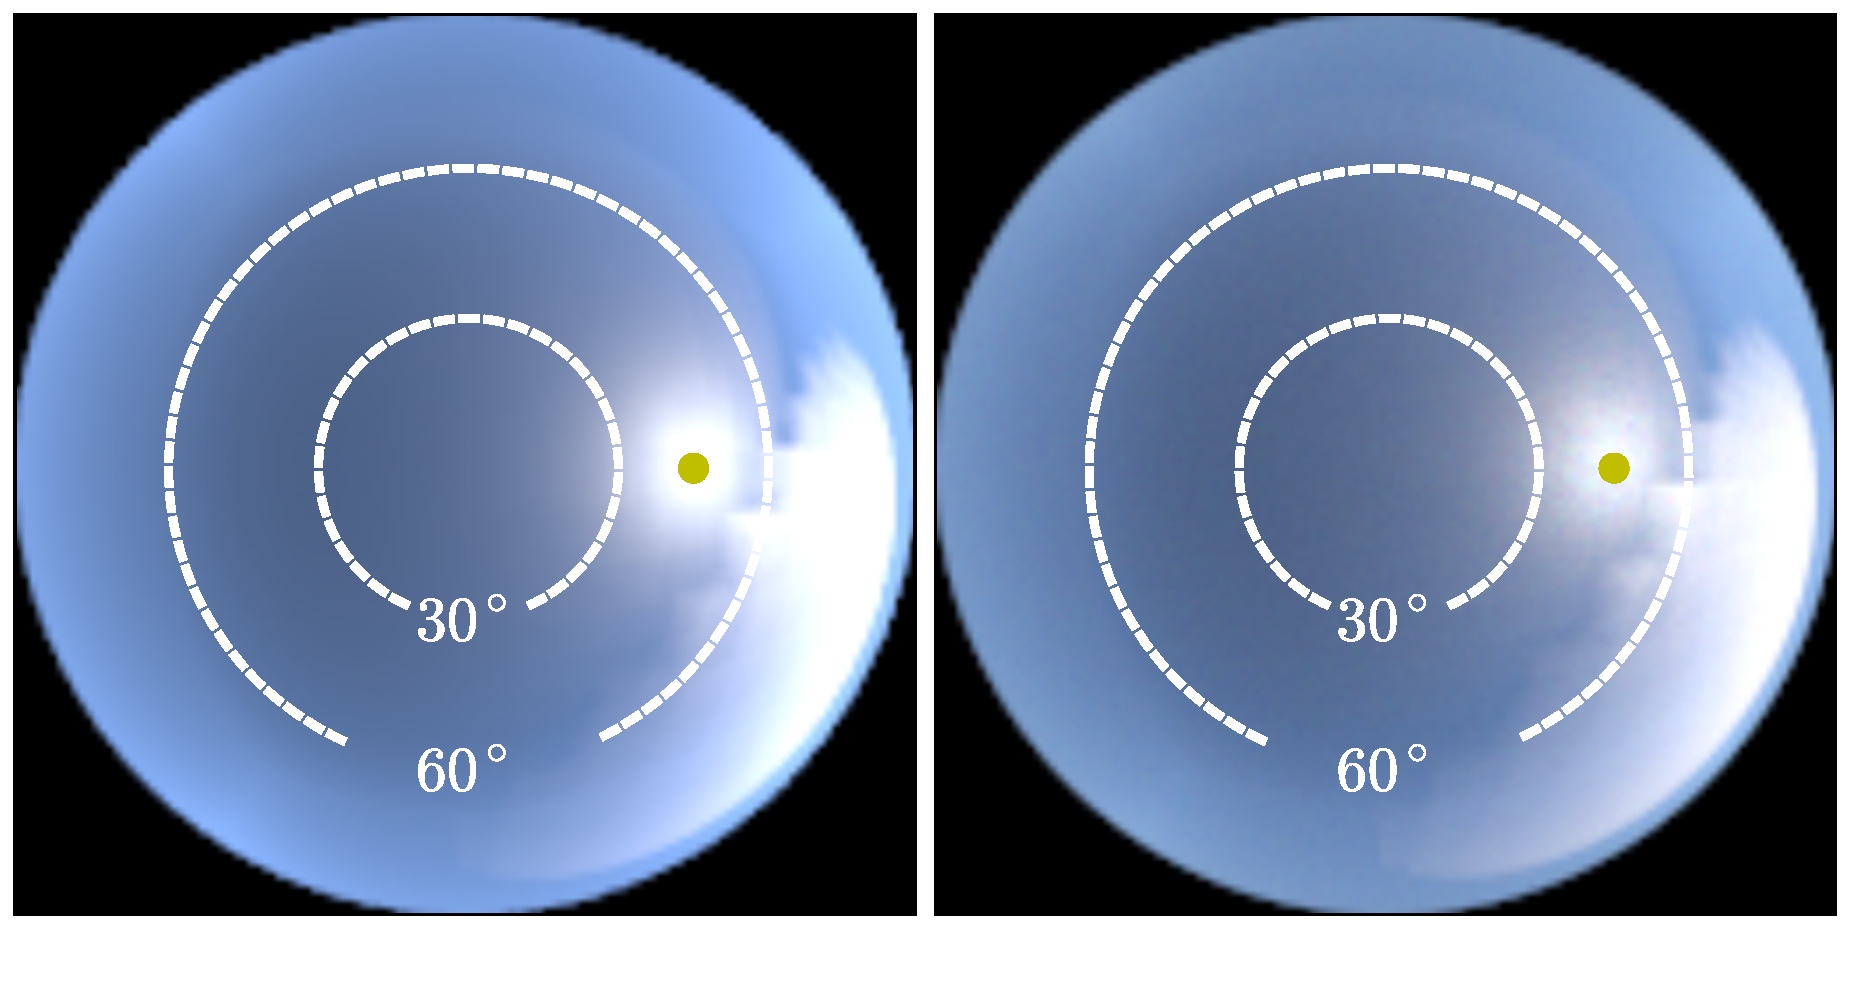
\includegraphics[width=\linewidth]{images/ref_images.pdf}}
  \caption{\small [a] Photograph of a sky that includes {\em Haze
      Blobs} rendered using the single-scattering model.  A yellow dot
    marks the Sun location. Dashed white circles mark elevation
    angles.  [b] Photograph of the same sky and view point rendered
    using the MC simulation (\cref{sec:monte-carlo-simul}).  [c] Cross
    section along the X-Axis of the MC simulation, Single-Scattering
    simulation and a Single-Scattering image created from the
    reconstructed distribution (\cref{sec:optimization-results}).}
  \label{fig:simulation-results1}
\end{figure}
To test the models, we simulated several atmospheric scenarios. Here
are the details:
\\

\noindent{\bf Sun}: The sun is at zenith angle $\Phi^{\rm
  SR}=45^o$. Its $L^{\rm TOA}$ is obtained
from~\cite{BBradiance,sun_composition}, with respective red-green-blue
ratios of $L^{\rm TOA}_{\rm R}:L^{\rm TOA}_{\rm G}:L^{\rm TOA}_{\rm
  B}=255:236:224$.
\\

\noindent{\bf Dimensions}: The sky domain has area of \SI{50 x
  50}{\km} extending from the ground up to altitude of
\SI{10}{\km}. This volume is divided into a rectilinear grid. We used
different grid sizes from \num{10 x 10 x 20} grid, where each voxel
has area of \SI{5 x 5}{\km} and vertical thickness of \SI{500}{\metre}
and up to \num{50 x 50 x 100} grid, where each voxel has area of \SI{1
  x 1}{\km} and vertical thickness of \SI{100}{\metre}.
\\

\noindent{\bf Aerosol}: We used particle-type 6 from the aerosol list
in Ref.~\cite{Martonchik2009}. This is a spherical non-absorbing
sea-salt/organic particle, whose anisotropy parameter per color
channel is $[g_{\rm R},g_{\rm G},g_{\rm B}]=[0.763,0.775,0.786]$. Its
corresponding extinction cross sections are $[\sigma^{\rm
  aerosol}_{\rm R}, \sigma^{\rm aerosol}_{\rm G}, \sigma^{\rm
  aerosol}_{\rm
  B}]=[16.5,16.2,15.9]$~\si[sticky-per]{\per\micro\meter\squared}.  At
all channels, $\varpi^{\rm aerosol}=1$.

We simulated various spatial distributions, as a product of two
functions. The first function is an exponential decay~\cite{Levi1980}
with altitude $h(k)$ of voxel $k$,
\begin{align}
  f_1[h(k)] = \sfrac{1} {n^{sea level}}
  \exp\left[-\sfrac{h(k)}{H^\mathrm{aerosol}}\right],
\end{align}
where $H^\mathrm{aerosol}=2$~\si{\km}. This expresses a general trend
of reduced atmospheric density with height.

The second function, $f_2$, expresses a clustered nature of aerosol
``clouds''. We define blobs in the form of 3D ellipsoids. There may be
multiple ellipsoids suspended.  Then
\begin{equation}
  f_2(k) =
  \left\{
    \begin{array}{ll}
      1  & \mbox{ if $k\in$ any blob cluster} \\
      0  & \mbox{ otherwise}
      \label{eq:f2}
    \end{array}
  \right.
  .
  \hspace{-0.05cm}
\end{equation}
The true aerosol distribution is then
\begin{equation}
  \label{eq:ntrue}
  {\bm n}^{\rm true}={\bm f}_1\odot {\bm f}_2  .
  \hspace{-0.05cm}
\end{equation}
As an example, we created a {\em Haze Blobs} scene using two ellipsoid
blobs (\cref{fig:results}a): the first is centered at altitude
\SI{3.3}{\km}, and has horizontal width of \SI{32}{\km} and vertical
thickness of \SI{2.8}{\km}. The second ellipsoid is centered at
altitude \SI{6.6}{\km}, and has lateral width of \SI{24}{\km} and
vertical thickness of \SI{2.1}{\km}. Note that the horizontal widths
are much larger than the vertical ones. This is consistent with scales
of atmospheric aerosol distributions.
\\

\noindent{\bf Cameras}: Each ground-based camera has a hemispherical
field of view, capturing the entire sky from its viewpoint. We used
different numbers of cameras ranging from 12 viewpoints to 100, on a
grid.  The resolution of each camera is low, expressing the fact that
cloudless (yet hazy) sky images are rather smooth.  For example,
\cref{fig:simulation-results1}a and \cref{fig:simulation-results1}b
show example photographs of the {\em Haze Blobs} scene as simulated by
the Single Scattering model and MC model, respectively, from the same
viewing point.  \cref{fig:simulation-results1}c compares a cross
section of the photographs along the horizontal Axis.

%%%%%%%%%%%%%%%%%%%%%%%%%%%%%%%%%%%%%%%%%%%%%%%%%%%%%%%%%%%%
%%%%%%%%%%%%%%%%%%%%%%%%%%%%%%%%%%%%%%%%%%%%%%%%%%%%%%%%%%%%

\section{Inverse Problem}
\label{sec:inverse-problem}

In this paper, we assume that the type of the aerosol above an area is
known~\cite{Martonchik2009}. Hence, we focus on estimating the density
distribution $\DistUnknown$.  At hand, we have $N_{\rm views}$
measured photographs $\{ {\bm i}^{\rm measured}_c\}_{c=1}^{N_{\rm
    views}}$. The recovery task is phrased as optimization of an
objective function that fits the image-formation model to the measured
photographs, under constraints. Let $\DistSet$ be the set of all
legitimate distributions, according to constraints.  Particularly,
$\DistUnknown$ is non-negative, and its spatial support is bounded
between the ground and the TOA. The optimization problem is
\begin{equation}
  \label{eq:minobjectiveA}
  \DistEstimated =
  \argmin_{\DistUnknown \in \DistSet} \CostFunc{\DistUnknown}
\end{equation}
where
\begin{equation}
  \label{eq:objectiveA}
  \CostFunc{\DistUnknown}
  = \sum_{c=1}^{N_{\rm views}}
  \left\| 
    \MaskSun[{\bm i}^{\rm measured}_c - {\bm i}_c({\bm n})]
  \right\|^2_2
  + \eta \Psi({\bm n})
\end{equation}
Here $\MaskSun$ masks the area around the sun, which in real-world
photographs is indeed blocked. %and the horizon.
% These regions are prone to dominant multiple scattering.
In Eq.~(\ref{eq:objectiveA}), $\Psi({\bm n})$ is a regularization term
that expresses some prior knowledge on the distribution, while $\eta$
is a regularization weight.

Since aerosol distributions are usually fuzzy, useful regularization
is by a {\em smoothness term}, which penalizes energy in second order
spatial derivatives (3D Laplacian), $\| \nabla^2{\bm
  n}\|^2_2$. Regularization is not required when data is sufficient
and reliable. As seen in Fig.~\ref{fig:groundgrid}, voxels at high
altitude have good coverage by many cameras at multiple directions,
while at low altitude voxels are mainly observed by local
cameras. Hence, regularization can be weakened with altitude. We
accomplished this weakening using a weight
$w(k)=\exp\left[-h(k)/H^\mathrm{smooth}\right]$.  Overall we use
\begin{equation}
  \label{eq:regularizer}
  \Psi({\bm n}) = \| {\bf W} \Laplacian{\bm n}\|^2_2
\end{equation}
where $\Laplacian$ is a matrix representation of the 3D Laplacian
operator, and matrix ${\bf W}$ is diagonal, whose elements are $w(k)$.

We solve~\cref{eq:minobjectiveA} using standard optimization tools.
The gradient of $F$ with respect to ${\bm n}$ is
\begin{align}
  \Grad{{\bm n}} F = -2\sum_{c=1}^{N_{\rm views}}
  \transpose{\left[{\bm J}_{{\bm i}_c}({\bm n})\right]} [{\bm i}^{\rm
    measured}_c - {\bm i}_c({\bm n})] + 2 \eta
  \transpose{\Laplacian}\transpose{{\bf W}}{\bf W}\Laplacian{\bm n}
  \;.
  \label{eq:gradient1}
\end{align}
Here the matrix ${\bm J}_{{\bm i}_c}({\bm n})$ is the Jacobian of the
vector ${\bm i}_c$ with respect to ${\bm n}$.  Element $(\Theta,k)$ of
this matrix differentiates the intensity in pixel ${\bm \Theta}$ (in
viewpoint $c$) with variation of the aerosol density at voxel $k$,
i.e., $\partial i_c({\bm \Theta})/\partial{n(k)}$.

We now detail the derivation of the Jacobian ${\bm J}_{{\bm i}_c}({\bm
  n})$. First, we provide some results relating to differentiation.
Let $\vect{a}(\vect{n}),\vect{u}(\vect{n})$ be vector functions: each
outputs a vector of length $r$. Let $\mat{C}$ be a $r \times N_{\rm
  voxels}$ matrix, where $N_{\rm voxels}$ is the length of ${\bm n}$.
Then,
\begin{align}
  \label{eq:partial1}
  \PartDeriv{\transpose{\mat{C}} (\vect{a} \odot \vect{u})}{\vect{n}}
  = \left[ \PartDeriv{\vect{a}}{\vect{n}} \OpDiag{\vect{u}} +
    \PartDeriv{\vect{u}}{\vect{n}} \OpDiag{\vect{a}} \right] \mat{C}.
\end{align}
Here $\OpDiag{\vect{v}}$ is a conversion of a general vector
$\vect{v}$ into a diagonal matrix, whose main diagonal elements
correspond to the elements of $\vect{v}$. Now, let
% \begin{align}
$\vect{a}(\vect{n}) = \exp(-{\mat{C}}\vect{n})$,
% \label{eq:example1}
% \end{align}
% In \cref{eq:example1},
where the exponent is element-wise (not raising an operator to some
power). Then
\begin{align}
  \label{eq:partial2}
  \PartDeriv{\vect{a}}{\vect{n}} &= - \transpose{\mat{C}} \,
  \OpDiag{\exp(-{\mat{C}}\vect{n})}.
\end{align}
Using \cref{eq:partial2},
\begin{align}
  \label{eq:partial4}
  \PartDeriv{\exp[-(\vect{\tau}_c^{\rm air} + {\sigma}^{\rm
      aerosol}{\bm D}_c {\bm n})]}
  {\vect{n}} &= - {\sigma}^{\rm aerosol}\transpose{\OpDistance_c} \,
  \OpDiag{\exp[-(\vect{\tau}_c^{\rm air} + {\sigma}^{\rm aerosol}{\bm
      D}_c {\bm n})]},
\end{align}
where $\vect{\tau}_c^{\rm air}$ is independent of ${\bm n}$. Using
\cref{eq:partial1},
\begin{align}
  \label{eq:partial3}
  \PartDeriv{\, [\varpi^{\rm aerosol}\sigma^{\rm aerosol} P^{\rm
      aerosol}_g(\vect{\Phi}^{\rm scatter}_c) \odot{\bm n}]}{\vect{n}}
  = \varpi^{\rm aerosol}\sigma^{\rm aerosol}\OpDiag{P^{\rm
      aerosol}_g(\vect{\Phi}^{\rm scatter}_c)}.
\end{align}
Based on \cref{eq:partial4,eq:partial1,eq:partial3} we derive the
Jacobian of \cref{eq:bigIA} in close-form,
\begin{align}
  % {\bm J}_{{\bm i}_c}({\bm n}) &= L^{\rm
  % TOA}(\abbrev{A}-\abbrev{B})\abbrev{C}
  {\bm J}_{{\bm i}_c}({\bm n}) &= L^{\rm TOA}{\sigma}^{\rm
    aerosol}({\bf A}-{\bf B}) \OpDiag{\exp[-(\vect{\tau}_c^{\rm air} +
    {\sigma}^{\rm aerosol} {\bm D}_c {\bm n})]}
  \transpose{{\vect{\Pi}}_c} ,
  \label{eq:gradient2}
\end{align}
where
% \begin{align}
%   \label{eq:gradient3}
%   {\bf A} &= \varpi^{\rm aerosol}
%   \OpDiag{ P_g^{\rm aerosol}(\vect{\Phi}^{\rm scatter}_c)} \nonumber\\
%   {\bf B} &= \transpose{{\bm D}_c} %\nonumber\\
%%   & \;\;\;
%   \OpDiag{[\tilde{\vect{\alpha}}^{\rm air}_c + \varpi^{\rm
%   aerosol}\sigma^{\rm aerosol} P^{\rm aerosol}_g(\vect{\Phi}^{\rm
%   scatter}_c) \odot{\bm n} ]}
%    %   \nonumber \\
%  %   \abbrev{C} &= \OpDiag{\exp[-(\vect{\tau}_c^{\rm air} +
%  %   {\sigma}^{\rm
%   %   aerosol} {\bm D}_c {\bm n})]} \transpose{{\vect{\Pi}}_c}
% \end{align}
\begin{equation}
  \label{eq:gradient3}
  {\bf A} = \varpi^{\rm aerosol}
  \OpDiag{ P_g^{\rm aerosol}(\vect{\Phi}^{\rm scatter}_c)}
  ,\;\;\;
  {\bf B} = \transpose{{\bm D}_c}
  \OpDiag{[\tilde{\vect{\alpha}}^{\rm air}_c + \varpi^{\rm
      aerosol}\sigma^{\rm aerosol} P^{\rm aerosol}_g(\vect{\Phi}^{\rm
      scatter}_c) \odot{\bm n}    ]}
\end{equation}


%%%%%%%%%%%%%%%%%%%%%%%%%%%%%%%%%%%%%%%%%%%%%%%%%%%%%%%%%%%%
%%%%%%%%%%%%%%%%%%%%%%%%%%%%%%%%%%%%%%%%%%%%%%%%%%%%%%%%%%%%

\section{Results}
\label{sec:optimization-results}

We applied the reconstruction algorithm \cref{sec:inverse-problem} to
the images simulated in \cref{sec:simul}. We used the L-BFGS-B
algorithm~\cite{BFGS} on a computer cluster. Each core was dedicated
to rendering a modeled image. The algorithm was initialized by ${\bm
  n}=0$. Satisfactory convergence occurred in several thousand
iterations, taking a couple of hours to complete in total.

An iso-surface visualization of the original {\em Haze Blobs}
distribution is shown in \cref{fig:results}a. \cref{fig:results}c show
the reconstructed scene based on images simulated by the Single
Scattering model. \cref{fig:results}e visualizes the reconstructed
scene based on images simulated by the MC model. The distributions
appear consistent, though there are errors that stem from the random
noise in the images. To quantify the results, we use a relative error
measure based on the $\ell_1$ norm
\begin{equation}
  \label{eq:ndiff}
  \epsilon=\frac{\| \hat{\bm n}  - {\bm n}^{\rm true} \|_1}
  {\| {\bm n}^{\rm true} \|_1} ,
\end{equation}
It is equivalent to the aerosol mass that is over and under-estimated
in all voxels, relative to the total aerosol mass in the scene.  In
the {\em Haze Blobs} case, $\epsilon=0.143$ and $\epsilon=0.646$ for
the reconstructions based on the Single-Scattering images and MC
images respectively. We used the distribution reconstructed based on
the MC images to create images using the Single-Scattering
model. \cref{fig:simulation-results1}c shows a cross of such an image
compared to the original MC image.

We created a {\em Haze Front} scene. \cref{fig:results}b shows an
iso-surface visualization of this distribution.
\begin{figure}
  \centering
  \yoavcomment{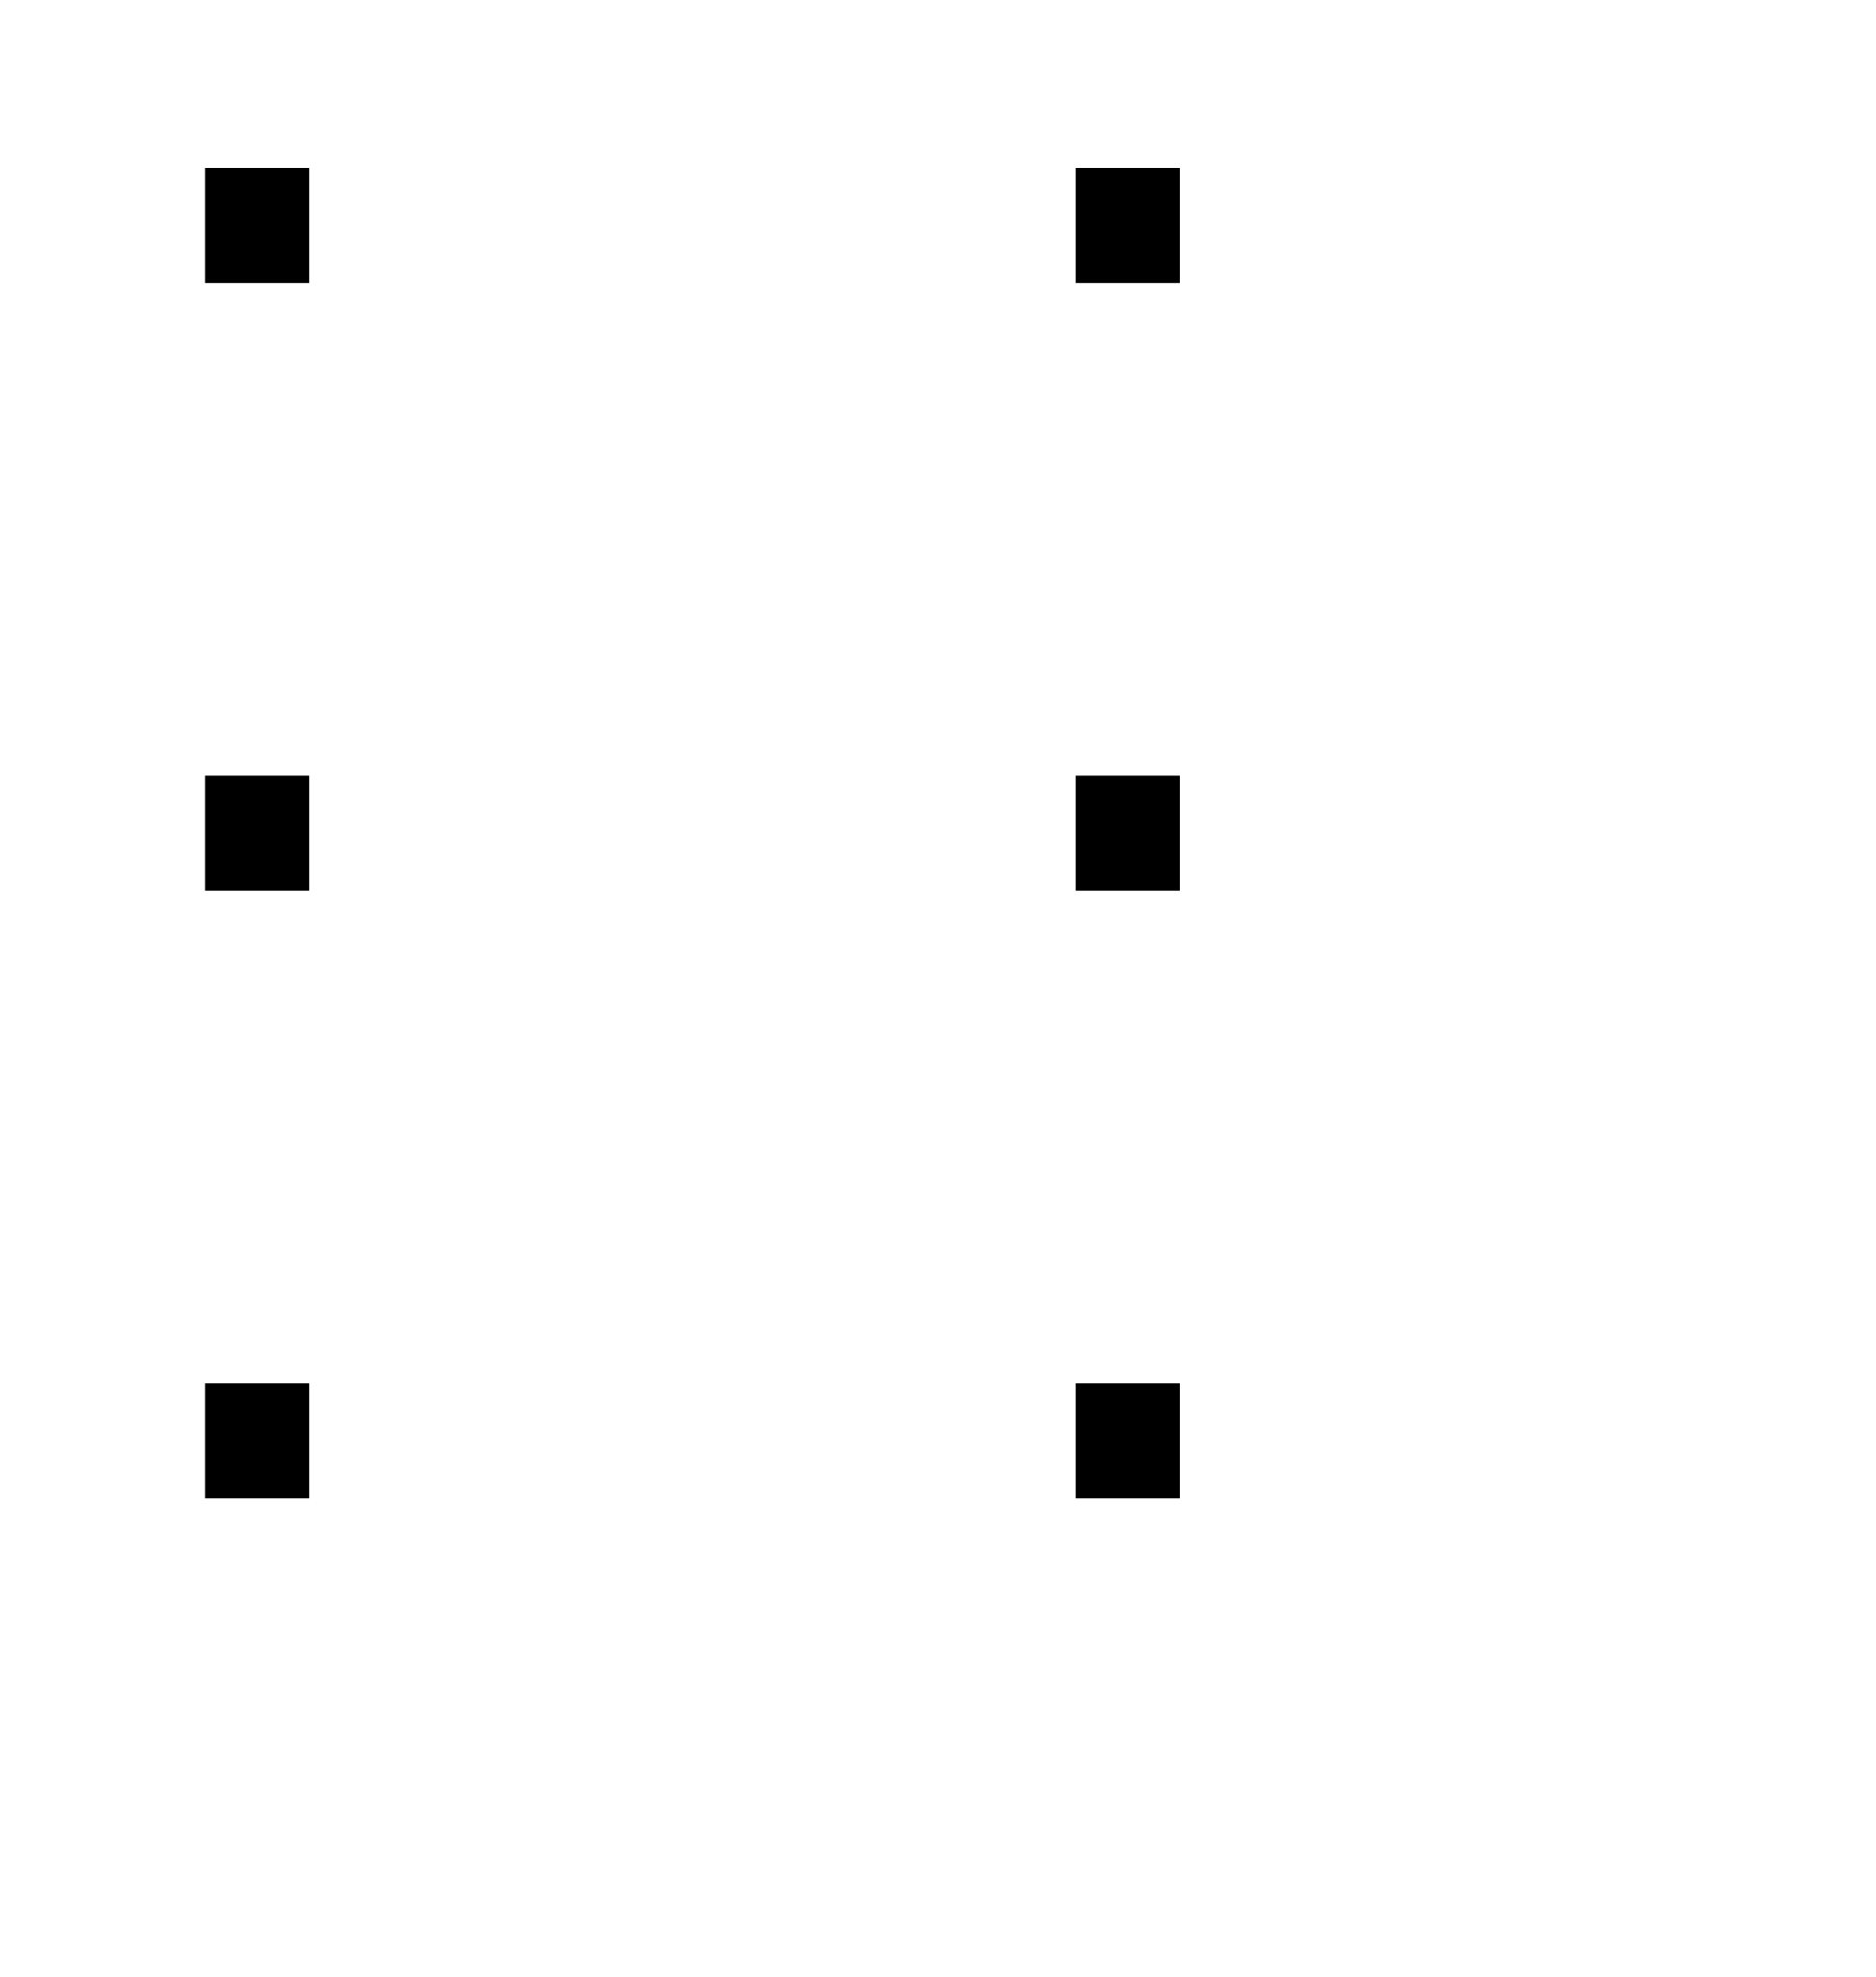
\includegraphics[width=\columnwidth]{images/results}}
  \caption{\small [a] and [b] Simulated 3D aerosol distribution
    composed of a {\em Haze Front} and {\em Haze Front}
    respectively. [c] and [d] Reconstruction of the same scenes when
    using Single-Scattering simulated images as input.  [e] and [f]
    Reconstruction of the scenes when using MC simulated images as
    input.  Color represents aerosol density. The density units are
    $10^{6}~{\rm particles}/{\rm m}^3.$}
  \label{fig:results}
\end{figure}
Here an ellipsoid degenerated to an elliptic cylinder that partly
enters the analyzed volume. It is centered at altitude \SI{5}{\km},
has vertical thickness of \SI{4}{\km} and length of \SI{32}{\km} (only
part of which enters the volume). The haze front stretches across the
width of the volume.  \cref{fig:results}d and \cref{fig:results}f
visualizes the recovered 3D distribution of this scene. For the {\em
  Haze Front}, $\epsilon=0.199$ and $\epsilon=0.654$ for the
reconstructions based on the Single-Scattering images and MC images
respectively.

%%%%%%%%%%%%%%%%%%%%%%%%%%%%%%%%%%%%%%%%%%%%%%%%%%%%%%%%%%%%
%%%%%%%%%%%%%%%%%%%%%%%%%%%%%%%%%%%%%%%%%%%%%%%%%%%%%%%%%%%%

\section{Conclusions}
\label{sec:conclusions}

We describe a new way to sense the 3D atmosphere. We show feasibility
of departing from common 1D aerosol distribution models, in favor of
detailed 3D analysis.  The paper describes both a novel data
acquisition system concept for this recovery task, and a dedicated
algorithm for reconstructing aerosol distributions.

Even without regularization, the reconstruction algorithm handles
arbitrary density distributions. Using more prior knowledge,
e.g. spatial smoothness will improve the recovery.  The algorithm uses
a single scattering model. This approximation is valid when the
optical depth is small, which is common. To handle dense atmospheric
conditions (smoke, clouds), multi-scattering must be incorporated.

The goal, of coarse, is to deploy such a system on a very large
scale. However, it must be first ensured that camera units are both
cost effective and field-robust, and that their positioning density is
proper. This will require a long-term engineering effort. Camera
specifications should be set to optimally recover a wide range of
aerosol distributions. This requires a major theoretic and numerical
research and development phase.  The new sensing modality and object
of interest offer a new domain for computational photography
problems. For example, how can compressed sensing principles be
employed here? How can priors be used to make data acquisition more
efficient? How can such a system be calibrated over time? Many such
questions and solutions would rise.


\end{document}

